\part{Proposed Solution}
    \chapter*{Overview}
        Considering all the problems explained previously, Reply proposed a solution for developing the Data Warehouse, as shown in figure \ref{fig:azure:workflow}.
        Their proposal also included a software architecture for performing analyses on the Data Warehouse.
        
        \begin{figure}
            \centering
            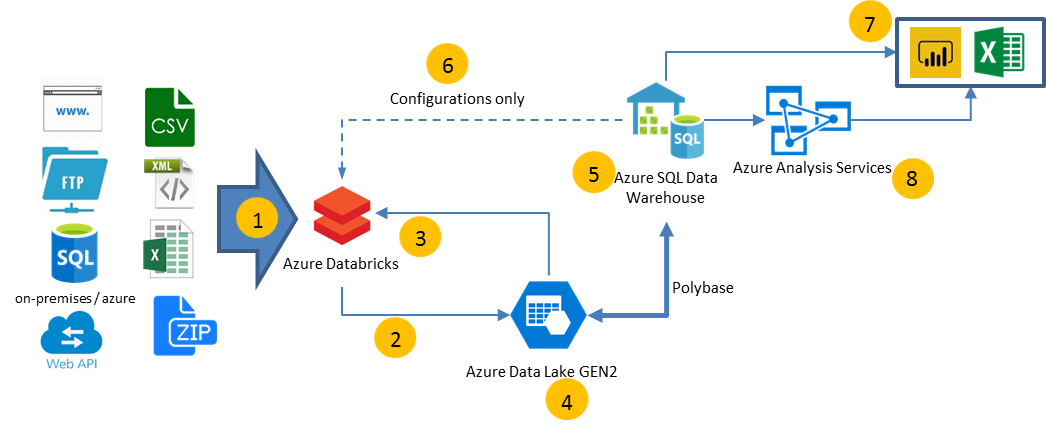
\includegraphics[width=\textwidth]{res/azure/workflow.png}
            \caption{Interaction between Azure components.}
            \label{fig:azure:workflow}
        \end{figure}
        
        \begin{enumerate}
            \item Several scripts, executed by Databricks, download the data using different techniques, such as API calling, FTP downloading or web scraping.
            \item This data is then stored on DataLake, under the \texttt{rawdata} folder.
            \item Those files are recovered by Databricks, which applies some transformations on the data, for example normalization or column removal.
            \item The result is saved again on DataLake, in \textit{csv} format, under the \texttt{srcdata} folder.
            \item The values from the \textit{csv} files are loaded into the data warehouse.
            The communication between the blob storage and the data warehouse is handled by Polybase.
            \item Some values stored in the data warehouse are accessed by Databricks and used as configuration settings.
            \item The data warehouse is queried by reporting tools, such as Excel or PowerBI, as well as algorithms developed by Axpo.
            \item In case of heavy workloads, it is also possible to query a copy of the data warehouse, located on Azure Analytics Services.
        \end{enumerate}
        
        I analyzed their proposal, paying particular attention to the ETL process and Data Warehouse structure, as well as the workflow chosen for developing such structures.
        
        In what follows, it will be discussed:
        \begin{itemize}
            \item The workflow used by Reply.
            \item How the ETL process works.
            \item The structure of the Data Warehouse and the reasons for that choice.
        \end{itemize}
        
        Problems and difficulties identified during each part of the process will also be discussed.
        Several examples will also be provided.

    \chapter{Migration Process} \label{section:organization}
        In this chapter we will analyze how the migration has been organized.

Several aspects will be seen, ranging from how the whole project has been split into smaller activities, called \textit{Sprints}, to the workflow used by Reply to develop each Sprint.

\section{Sprints}
    \label{section:sprints}
Reply proposed to organize its migration work into Sprints.

A \textbf{sprint} can be defined as a set of activities needed to migrate an existing process.
A sprint is comprised of several data streams from multiple providers.

A \textbf{provider} is a data source, usually external, from which data is retrieved and stored on the Axpo Data Warehouse.

A \textbf{data stream} is a specific kind of data exposed by a given provider.

\subsection{Introduction}
    The data warehouse needs to contain data originating from a large amount of providers.
Each provider exposes information related to a specific aspect (for example, stock prices or gas consumption).

The amount of data needed is very large, reaching up to a few thousand different data streams across all providers.
Considering the size of the project, it was necessary to organize the ETL development of all data streams.
This organization was driven by two factors.

First of all, it was necessary to migrate multiple existing processes, prioritizing specific ones.
Some processes played a critical role in the company and having them on a more robust and efficient structure would have provided a greater benefit.

Secondly, each tool requires a different set of data streams, with an almost non-existent overlap.
As such, each process could be migrated independently.

\paragraph{Example}
    A specific tool extracted data from existing on-premise databases to produce market prices reports.
    Since the databases were going to be migrated to the cloud, it was necessary to create a cloud-based ETL process for all the data used by these tool.
    
    The development of a new ETL process was necessary to keep the Data Warehouse populated with the most recent data.
    Having recent data was a critical requisite, since up-to-date information are needed on a daily basis by multiple Axpo employees.

    As such, we planned a Sprint with the goal of enabling the tool to fetch all of its data from the Data Warehouse, instead of having to query multiple on-premise databases.

    For this sprint it was necessary to download a total of 372 data streams from 9 different providers.
    
    Each provider exposes multiple data streams.
    For example, GME\footnote{
        GME is the manager of the Italian Spot Electricity Market.
        For more information, see appendix \ref{section:providers:gme}.
    } provides data about different market sessions, ranging from MGP to all the MI sessions.
    Moreover, different kinds of information are provided for each session, such as prices, quantities, and transit limits.
    
    Each file has been considered a separate data stream.
    
\subsection{Balancing}
    Sprints have been designed to be balanced, i.e., each sprint requires roughly the same amount of effort.

It is necessary to take into account different factors, in order to estimate the effort required for a sprint, as well as the expected sprint deadline.

This balancing activity depends on the following aspects:
\begin{itemize}
    \item Provider source
    \item Technique required to download data
    \item Intrinsic provider complexity
\end{itemize}

These factors are fundamental from an organizational point of view, since they allow Axpo employees to coordinate their work with the Data Warehouse development process.

For example, some employees have processes currently running on local machine, which they want to transfer to the cloud.

In order to transfer they processes they need, however, to retrieve data from the Data Warehouse.
As a consequence, they need to wait for the ETL process to be fully developed before they can start migrating their processes onto the Cloud.

\subsubsection{Provider source}
    An important aspect to consider when estimating the complexity of a provider is whether it is an internal or external source.
    
    \begin{table}
        \centering
        \begin{tabular}{|c|c|c|}
            \toprule
                                            & Internal              & External                  \\
            \midrule
             Already known                  & Yes, in depth         & Sometimes, not in depth   \\
             Can be modified                & Yes                   & No                        \\
             Direct access to DB            & Yes                   & No                        \\
             Possible data inconsistency    & Yes, but known        & Yes, unknown              \\
             \bottomrule
        \end{tabular}
        \caption{Difference between internal and external data sources.}
        \label{tab:reply:sprints:data_source}
    \end{table}
    
    \paragraph{Internal}
        Internal sources are directly owned, and often also developed, by Axpo.
        They can be either databases or tools.
        
        Internal sources are the easiest to extract data from, for a variety of reasons.
        
        First of all, they are already well-known, since they have been developed or chosen (in case of a third-party tool) by someone working at Axpo.
        
        Secondly, they can be modified to accommodate the Data Warehouse needs.
        For example, if the Data Warehouse needs to extract data in a specific format, it is possible to modify the tool to expose it in that given format.
        As such, the Data Warehouse extraction process can be simplified.
        
        Another important aspect is that most of these tools rely on its own database, which can also be directly queried to extract information directly, thus further simplifying the process.
    \paragraph{External}
        Most providers can be defined as external sources, that is websites or services not owned by Axpo.
        
        Some of these services are public, while others provide data under a paid subscription.
        
        These websites present several difficulties, compared to internal sources.
        
        First of all, they are less known that internal sources, since no-one at Axpo directly worked on them.
        As a consequence, it is necessary to spend more time studying the tool.
        There is also a consistent possibility of unexpected issues coming up during development\footnote{
            For example, a provider exposes data pertaining to the current year in \texttt{csv} format, while data related to previous years are stored in \texttt{gz} format.
            There is however no documentation about this difference and the problem can only be noticed by analyzing when a custom downloader stops working.\\
            For a more in-depth description of the issues encountered, see section \ref{section:etl:difficulties}.
        }.
        
        Secondly, there is a lack of standardization between each source: each company provides data in its own format and way, making the extraction process more complex.
        
        Moreover, there could also be some problems with the data provided.
        For example, some providers use different date conventions depending of the type of data required.
        These different formats need to be normalized into a common notation before inserting the data into the Data Warehouse.\newline
        
    Table \ref{tab:reply:sprints:data_source} sums up the main differences between internal and external data sources.
        
\subsubsection{Download technique}
    Another important aspect to consider when estimating the complexity of a provider is the technique required for extracting data from it.
    
    A more complex extraction process will take more time and resources, and needs to be accounted for in advance.
    
    Also, some developers are more experienced than others on a particular extraction technique.
    To maximise efficiency, it is best to have each developer working on the technique they are more skilled in.
    
    This approach requires however having in a single sprint several different extraction techniques.
    Otherwise, some developers would be forced to work with technologies they are less familiar with, increasing the effort required for implementing the process.
    
    \paragraph{Database}
        Databases are the fastest and easiest sources to extract data from.
        
        Data are already in a structured format, since they are stored in a relational table.
        This structure can also be easily altered by writing a query, for example for aggregating or de-aggregating some data.
        
        The only difficulty is understanding the structure of the tables.
        However, since all databases are internal sources, this problem can easily be simplified by asking directly the Axpo employees who work on that database.
    
    \paragraph{FTP}
        Extracting data from FTP shares has a small degree of complexity.
        
        In most cases, the FTP shares store data in structured formats, such as \texttt{csv} or \texttt{xml}.
        
        To download data it is necessary to connect to these share points and retrieve the files required.
        
        These files are then parsed and normalized depending on the data structure used by the provider.
        
        In some cases, these files require some special processing for the first lines, which are used as headers.
        
    \paragraph{API}
        Some websites offer an API service which can be called to extract data.
        
        Depending on the amount of documentation available, this process can either be considered as difficult as extracting data from an FTP share or can prove some serious challenges.
        
        In some cases, the required queries required are complex and require an extensive analysis of all parameter combinations, which can often only be carried out empirically.
        
    \paragraph{Web scraping}
        The most difficult and time consuming ETL approach is web scraping, which simulates human web site navigation.e
        
        Given its complexity, web scraping is chosen only as a last resort, when a website does not expose any service for directly extracting the data.
        
        Web scrapers not only require a large amount of time to be developed, but are also very susceptible to website changes: a single element moved a different page can break the download process for the whole provider.
        
\subsubsection{Provider complexity}
    An important factor to consider is also the intrinsic complexity of a given provider.
    
    Some providers consistently provide data in formats which are hard to parse or to extract.
    
    In some cases, some websites are difficult to navigate, requiring navigation of multiple pages just to find the information required, while others may require some functionalities (such as scrolling a page with a web crawler) which are hard to implement.
    
    In other cases, the data extracted may be in a format which is difficult to parse or requires complex transformation operations for obtaining a format suited for the Data Warehouse.
    
    These considerations, which apply at provider-level, are used to estimate a coefficient, which is applied to all the data streams of a given provider.
    This coefficient helps in correcting the time estimation for a given sprint.
    
\section{Process}
    This chapter will provide a description of how Reply organized the development of each sprint.

The initial organization presented a few problems, for which both I and the Project Manager requested some changes.

Both these problems and the changes will be analyzed as well as the limitations of the chosen workflow.

\subsection{Phases}
    The development of a sprint is composed by multiple phases, as shown in figure \ref{fig:reply:workflow}.

\begin{figure}
    \centering
    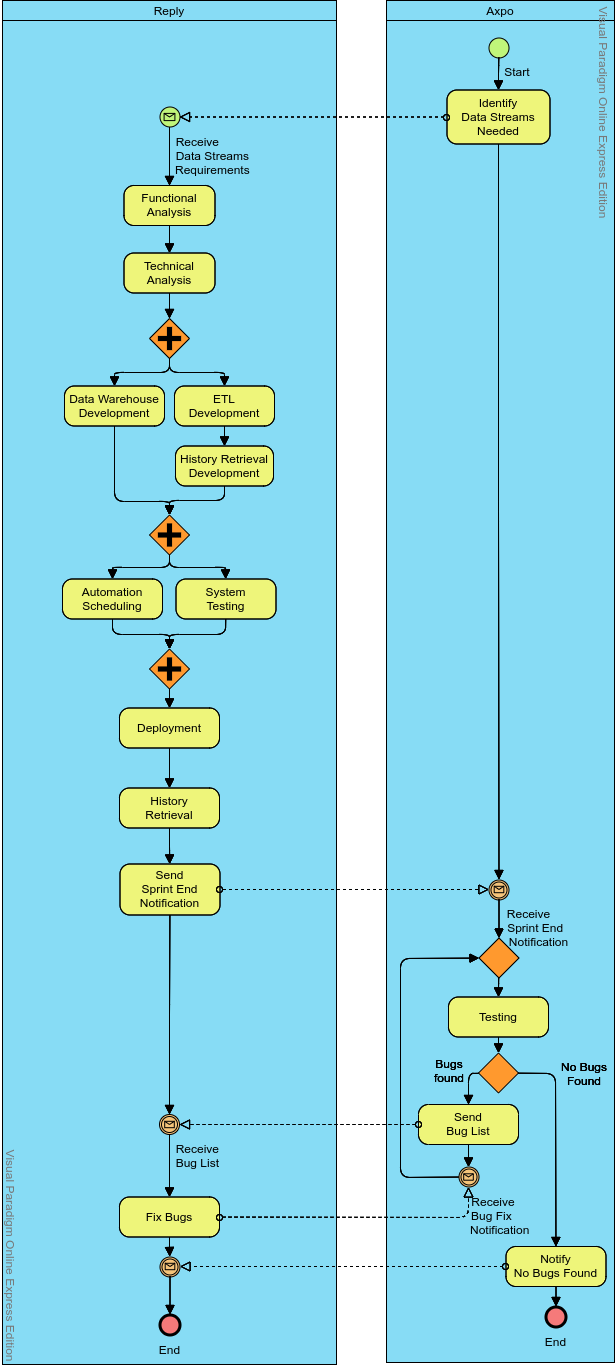
\includegraphics[width=\textwidth,height=\textheight,keepaspectratio]{res/reply_workflow.png}
    \caption{Workflow used by Reply.}
    \label{fig:reply:workflow}
\end{figure}

\paragraph{Functional analysis}
    \input{tex/chapters/2_solution/reply/workflow/phases/functional_analysis.tex}
\paragraph{Technical analysis} 
   \input{tex/chapters/2_solution/reply/workflow/phases/technical_analysis.tex}
\paragraph{ETL development}
    \input{tex/chapters/2_solution/reply/workflow/phases/etl_development.tex}
\paragraph{History retrieval development}
    \input{tex/chapters/2_solution/reply/workflow/phases/history_retrieval_dev.tex}
\paragraph{Data Warehouse design} 
    \input{tex/chapters/2_solution/reply/workflow/phases/dwh_design.tex}
\paragraph{Automation scheduling}
    \input{tex/chapters/2_solution/reply/workflow/phases/automation.tex}
\paragraph{System testing}
    \input{tex/chapters/2_solution/reply/workflow/phases/system_test.tex}
\paragraph{Deployment to production environment}
    \input{tex/chapters/2_solution/reply/workflow/phases/deployment.tex}
\paragraph{History retrieval}
    \input{tex/chapters/2_solution/reply/workflow/phases/history_retrieval.tex}
\paragraph{User Acceptance Test}
    \input{tex/chapters/2_solution/reply/workflow/phases/acceptance_test.tex}
\subsection{Issues}
    Several issues with the workflow have been found during development.
This section will list them, along with the chosen solutions.

\subsubsection{History Retrieval}
    Initially, the history retrieval process suffered from many unexpected issues.
    
    This phase was originally planned after the deployment process.
    However, during the first sprint, the retrieval process for many providers broke.
    
    Upon further analysis we discovered that several providers changed data format over the course of the years.
    As such, it was necessary to modify the history retrieval process to handle these special cases.
    
    For example, a specific provider exposes \texttt{csv} files for the current year and \texttt{gz} archives for the previous years.
    This difference had been overlooked during development since the developers only focused on recent files.
    
    After deployment, when the process had been scheduled to retrieve data for multiple years, the downloader crashed since it was expecting a \texttt{csv} file but retrieved an archive.
    Developers had to manually analyze the error log, as well as the provider website to understand the problem and implement a solution.
    
    Some other providers maintained instead the \texttt{csv} format, but changed their internal structure, for example adding or removing columns which were expected by the downloader.
    
    \paragraph{Optimization}
        As an additional safety measure, Reply decided to further modify the history retrieval process, making it download each day independently.
        
        Originally, the process downloaded all days required from the provider, before storing them in bulk onto the Data Warehouse.
        In case of errors all data downloaded would be lost.
        
        Since the errors related to different formats for old data have no impact on more recent data, it is reasonable to store each day independently onto the Data Warehouse.
        In this way, in case of errors, all the other information would still be available onto the Data Warehouse.
        
        This optimization also prevented the downloader from having to retrieve the same data multiple times in case of failure.
    
    \paragraph{Workflow change}
        This additional work caused some delays in the original planning, since they hadn't been originally taken into account.
        
        In order to take these delays into account, Reply decided to execute a preliminary history retrieval process during development, testing the process not on just a few days but on several years.
        In this way, this kind of errors would be noticed before deployment, ensuring the deadlines would be respected.
        
\subsubsection{Initial delays}
    The development of the first sprint took far more time than originally planned.
    
    This was caused by a misestimation of the ETL development complexity.
    This error was mainly caused by two factors.

    \paragraph{Technology}
        The team was not yet familiar developing on \textit{Microsoft Azure Cloud Computing Platform \& Services}.
        
        This aspect had been underestimated by Reply, which led to a too much optimistic deadline.
        Much more time than expected had been spent trying to solve problems related to Azure tools, which led to delays in the original planning.
        
    \paragraph{Providers}
        Another aspect which had been originally underestimated was the high complexity of some providers.
        
        Some providers required very complex methods to extract data from them.
        These methods required more time to develop than originally estimated, which led to more delays.\newline
    
    Since we requested Reply to respect the original deadlines even considering their delays, they had to add some team members to catch up, as well as grouping together some smaller sprints, to reduce the overhead.
    

% \subsection{Limitations}
    \subsubsection{Automated tests}
    Reply decided not to create automated tests but to rely on user tests instead.
    
    They stated that in the energy market scenario, users tests are more appropriate than automated tests for a variety of reasons.
    
    First of all, these data are very domain-specific, so writing a proper testing suite would require extensive domain knowledge.\\
    Secondly, most values come from external providers, so it is not possible to perform many actions if these values are detected as incorrect.\\
    Lastly, there is a notification system in place in case of critical errors (i.e. processes breaking and failing to complete).
    Reply has considered this notification system enough for this project.
    
    Further tests, such as the ones described in section \ref{section:tests:data}, have clearly shown that relying only on notifications and System Tests is not enough to assure the quality of the Data Warehouse.
    As a consequence, Reply has been requested to develop these tests during development, to shorten the delay between the deployment and the actual beginning of the data quality tests.
    
\subsubsection{Data correctness definition}
    An interesting aspect is the impossibility to determine if the data received are correct or not.
    
    Most data received are measurement taken by either operators or automated tools.
    In some other cases, data are the result of forecasting algorithms, developed by the provider themselves.
    
    Since there is no way to assert the correctness of the data received by the providers, the values shown on their websites are assumed to be correct.
    
    The only test that can be done is asserting that the information stored in the Data Warehouse, at the end of the download process, is identical to the information present on the websites.
    
\subsubsection{Priority vs non-priority data streams}
    All data streams have been categorized as priority or non-priority.
    
    Priority streams contain data needed by tools currently in use by the company.
    Having this data available is fundamental for running these tools on the cloud.
    
    On the other hand, some data has been marked as non-priority.
    These information are not currently used by any tool, but may be used in the future or for exploratory analysis.
    
    Given the low importance of having these data available in a short time, the only operation performed on them has been functional analysis, to identify if there are any issues with the data.
    A development date has, however, not been fixed: the ETL processes for these data stream will be developed during spare time or after all other priority data streams have been completed.
    
    The downside of this categorization is the lack of a precise time estimation for all the data streams.
    This is likely not to cause a consistent delay for a few data streams, but could become a problem for a high number of streams.
    
    Moreover, in several occasions Axpo employees had erroneously marked some data streams as non-priority, causing some confusion and forcing Reply to re-plan their work schedule.
    Changing these requirements naturally comports some delays, since we are requesting more work to be done before a deployment.
    
\subsubsection{Lack of formal documentation}
    A problem present in all development phases is the lack of a clear and formal documentation.
    Most of the information are in the heads of the developers, meaning that other people have either to ask them or to look directly at the code.
    The documentation present is represented in a non-clear way, usually using Excel sheets to annotate different types of information and comments.
    
    A more formal notation has been used, on the other hand, to represent the Data Warehouse structure.
    This notation, shown in Figures \ref{fig:reply:issues:dwh_diagram} and \ref{fig:reply:issues:dwh_diagram_table}, describes, however, only the columns present in each table, without specifying any relationship between them.
    Moreover, there is no clear distinction between fact tables (all the large boxes shown at the center of the Figure) and dimension tables (some of the small ones on the edges).
    
    \begin{figure}[p]
        \centering
        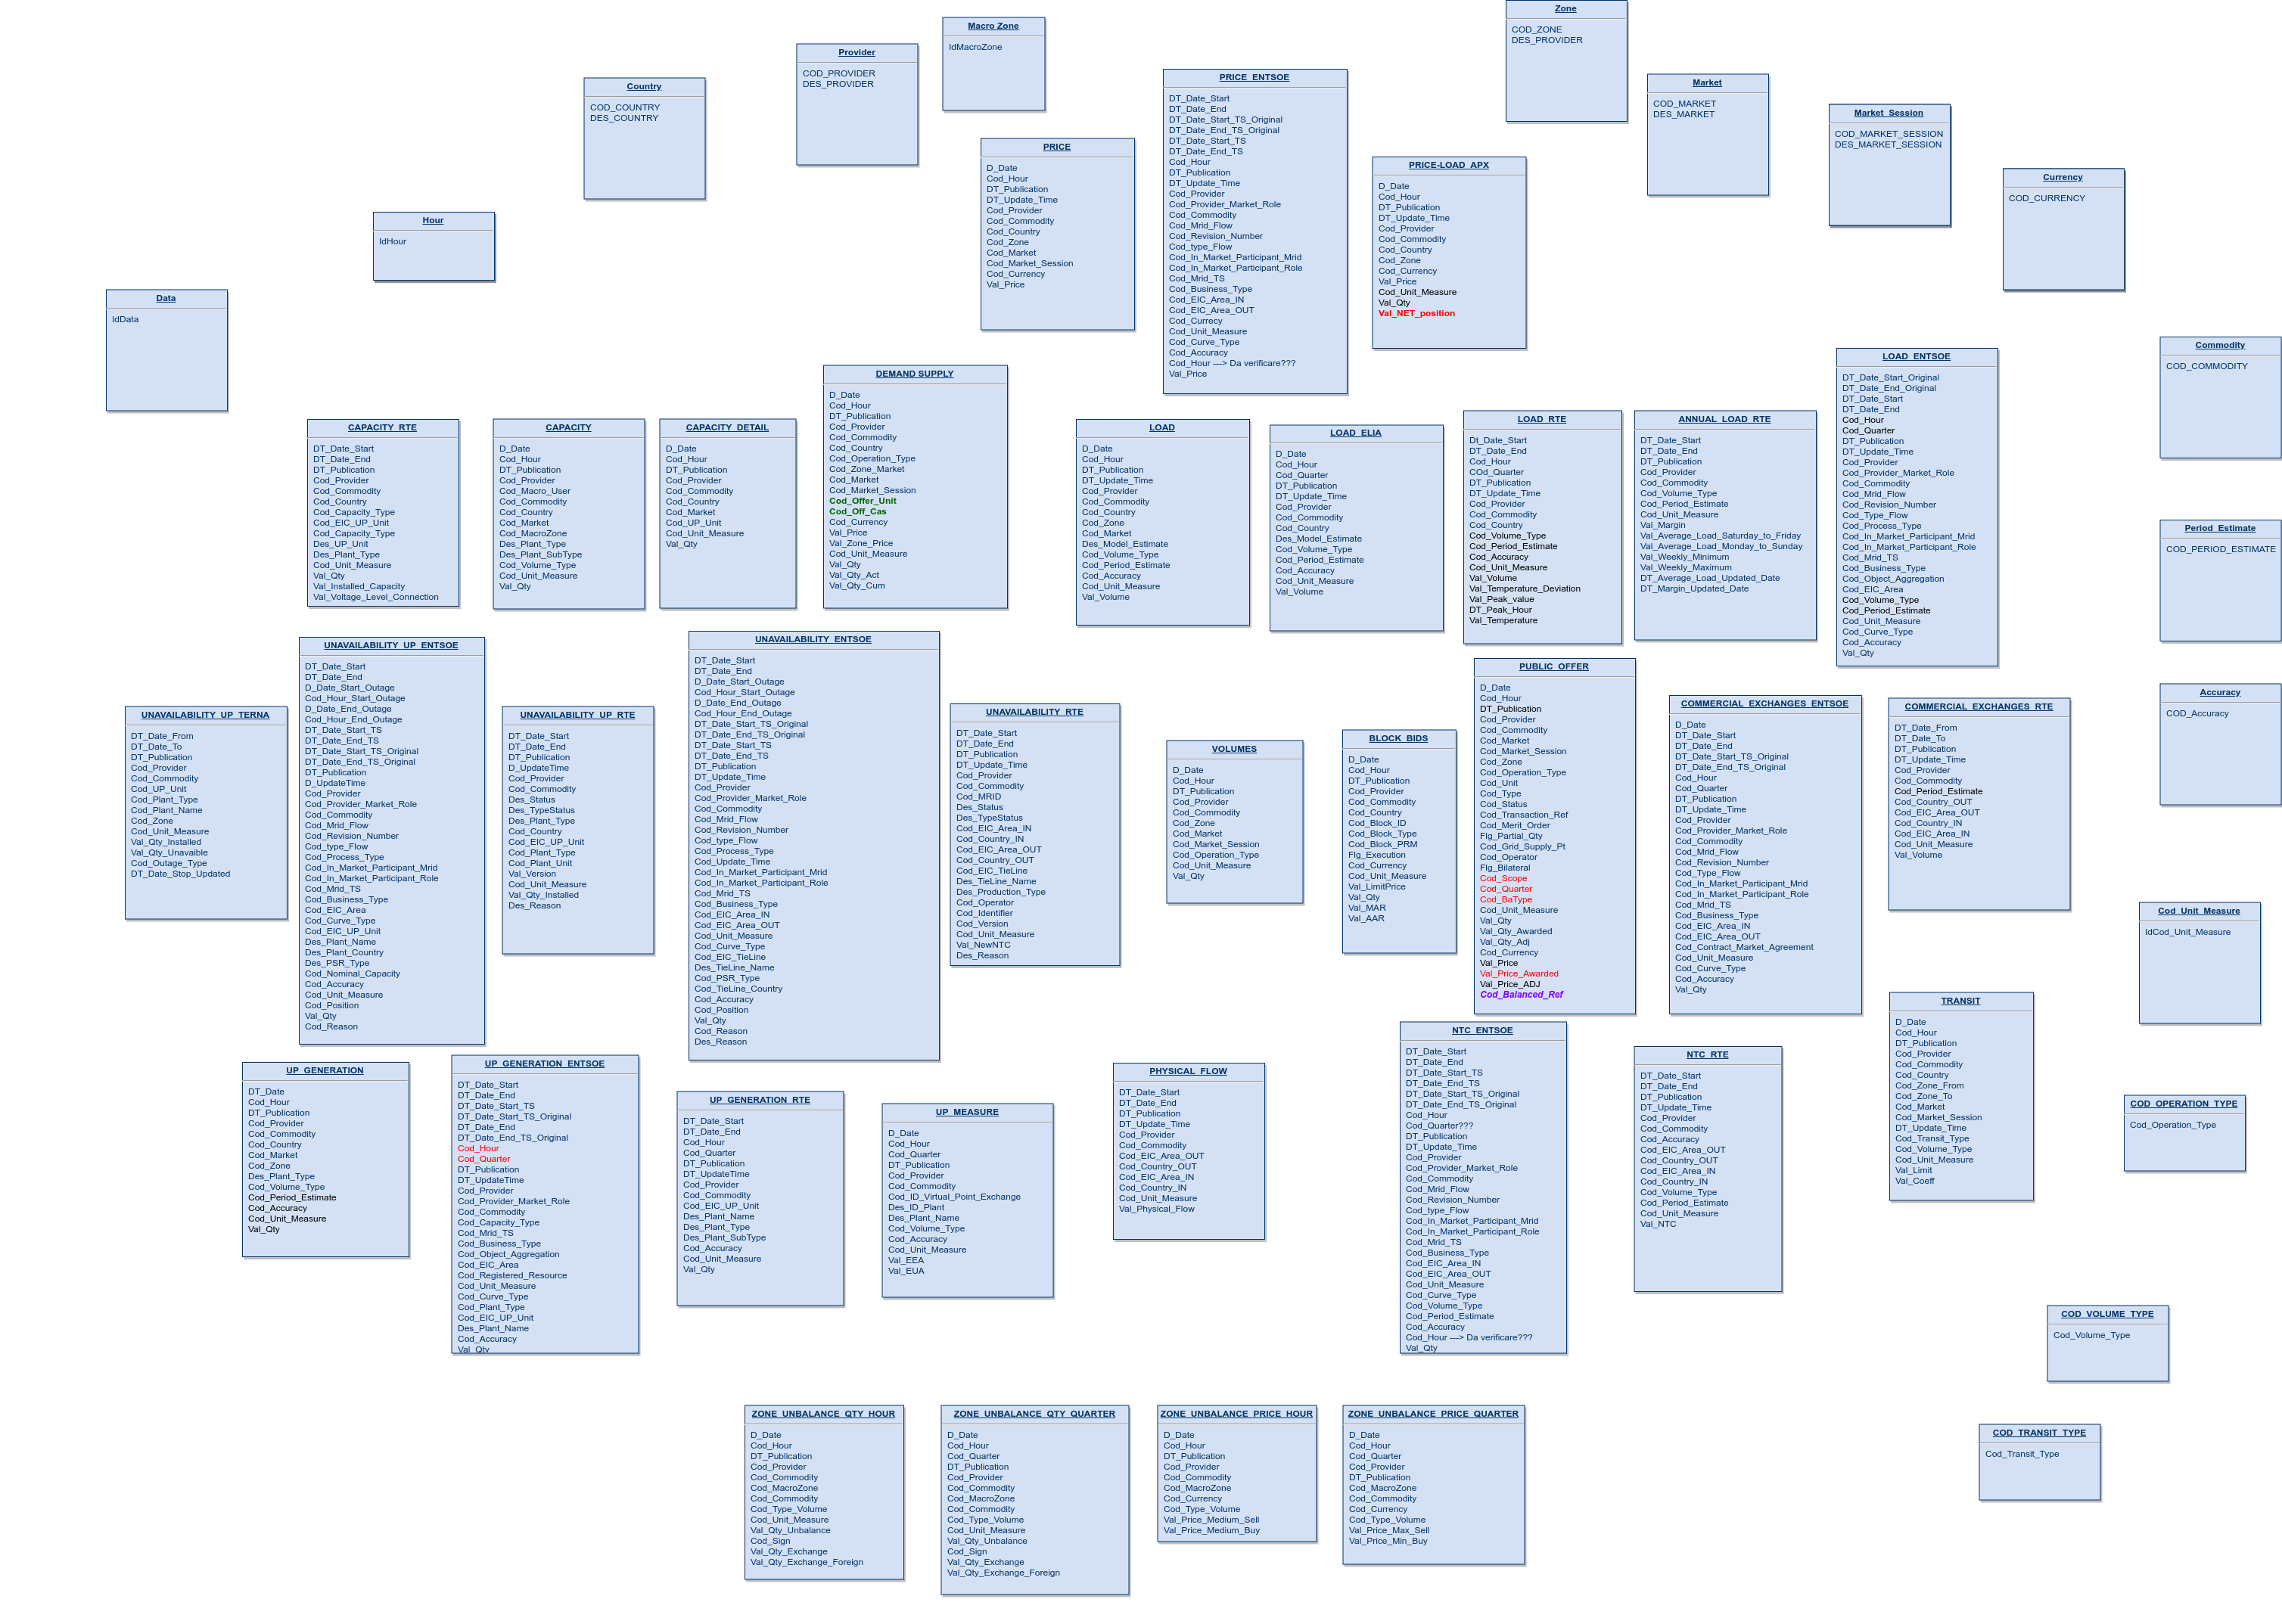
\includegraphics[width=\textwidth]{res/dwh_diagram.png}
        \caption{Diagram used for representing Data Warehouse structure.}
        \label{fig:reply:issues:dwh_diagram}
    \end{figure}
    
    \begin{figure}[p]
        \centering
        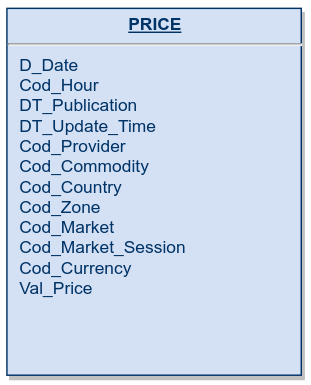
\includegraphics[width=.35\textwidth]{res/dwh_diagram_price.png}
        \caption{A single table from the Data Warehouse structure diagram.}
        \label{fig:reply:issues:dwh_diagram_table}
    \end{figure}
    
    An additional issue is that only the column names are reported, as shown in Figure \ref{fig:reply:issues:dwh_diagram_table}.
    Other relevant information, such as the data type for each column, are not shown.
    
    This design can, as a consequence, lead to confusion.


    \chapter{ETL Process}
        \label{section:etl}
In this chapter we will describe the process used for extracting, transforming and loading data into the Data Warehouse.

I analyzed the multiple problems encountered during the ETL development as well as the process employed by Reply.
Most problems were however solved by Axpo specialists, since their specific knowledge was required.

I also asked Reply to keep track of all the issues encountered as well as their status.

This can be used both by Reply, to better organize its work, and by Axpo, to understand if a delay is due to an unexpected issue and how well Reply is performing.

The resulting document can be used both as a small layer of documentation and to produce some tests for the more vulnerable parts of the ETL processes.

\section{ETL Operations}
    This section will provide a description of the main operations performed by the ETL process.
An exhaustive list is not provided, since describing each operation of them would be extremely long and repetitive.

\subsection{Extraction}
    Most processes are executed daily, so the downloaders usually retrieve files only for the current day.
    However the downloaders can also be easily configured to retrieve a range of dates, in case of history retrieval (which is only used to initialize the Data Warehouse).
    
    Each downloaded file is saved to the \texttt{rawdata} folder on DataLake \textit{as-is}.
    
    \subsubsection{Provider types} \label{section:etl:provider_types}
        Different download techniques are used, depending on the kind of services exposed by a particular provider.
        
        \paragraph{FTP}
            Several providers provide an FTP share, where they upload a few files each day, which contain the data for that given day.
            
            In this case the downloader just needs to connect to the FTP server and retrieve the files.
            
            Files stored here are usually either in \texttt{csv}, \texttt{xml} or \texttt{xls} format.
            
        \paragraph{API}
            Other websites provide an API which can be queried for data.
            
            The resulting datasets are usually in \texttt{json} or \texttt{xml} format.
            
            In this case the downloader makes several calls to the API, each one with different parameters.
            
        \paragraph{SQL databases}
            These providers provide the easiest interface, since it is possible to directly perform queries and extract the data in nearly any format.
            
            Since most of these providers are internal services owned by Axpo, their number is limited, compared to all the public providers.
            
        \paragraph{Web scraping}
            Some websites do not expose their data through any particular service.
            
            In this case the only solution is to build a web scraper, which simulates human web navigation retrieving information manually.
            
            This approach is the most complex and time consuming, since it has to be build \textit{ad hoc} for the website.
            Moreover, its re-usability across different websites is low, if non-existent, so it needs to be developed each time from scratch.
        
\subsection{Transformation}
    Databricks retrieves the files saved on \texttt{rawdata} and performs some operations on them, before saving the resulting datasets in \texttt{.csv} format on the \texttt{srcdata} folder in DataLake.
    
    The most commonly executed operations are:
        \begin{itemize}
            \item Reading the dataset: depending on its format different methods are needed
            \item Renaming columns
            \item Dropping unneeded columns
            \item Appending the file download date to each row, where not already present
            \item Unpivoting the dataset, if needed
            \item Normalizing column names
        \end{itemize}
        
    \paragraph{Unpivoting}
        A consistent number of datasets provide a value for each hour in a day in an apposite column.
        
        It is necessary to change the format, displaying on one column the hour and in another one the value.
        This operation is called \textit{unpivoting} or \textit{melting}.
        
        \begin{table}
            \centering
            \begin{tabular}{|c|c c c c c|}
                \toprule
                 Zone  & H1 & H2 & H3 & ... & H25   \\
                 \midrule
                 North & 12 & 15 & 14 & ... & 0     \\
                 South & 32 & 29 & 28 & ... & 0     \\
                 \bottomrule
            \end{tabular}
            \quad
            \begin{tabular}{|c|c c|}
                \toprule
                 Zone  & Hour  & Value   \\
                 \midrule
                 North & H1    & 12     \\
                 North & H2    & 15     \\
                 North & H3    & 14     \\
                 North & ...   & ...    \\
                 North & H25   & 0      \\
                 South & H1    & 32     \\
                 South & H2    & 29     \\
                 South & H3    & 28     \\
                 South & ...   & ...    \\
                 South & H25   & 0      \\
                 \bottomrule
            \end{tabular}
            \caption{Normal (left) and unpivoted (right) tables.}
            \label{tab:etl:melt}
        \end{table}
        
        Table \ref{tab:etl:melt} provides an example of unpivoting.
        In the left table we have 26 columns, one representing the zone and a column for each hour\footnote{There are 25 hours to account for DST.}, while in the right table we have 3 columns: zone, hour and value.
    
    \paragraph{Column names normalization}
        Some columns do not respect the naming convention decided for the Data Warehouse.
        
        Some columns may contain special characters or spaces, which cause problems when inserted into a database table.
        
        Several operations are performed to remove or replace these characters.
        
        For example, spaces and dashes are replaced with an underscore, parentheses of any type are removed and the character \code{\&} is replaced with its literal representation \code{and}. \\
        Also, all names are converted into lowercase.
            
\subsection{Loading}
    Databricks retrieves the files from \texttt{srcdata} and loads the data onto the Data Warehouse.
    
    The Data Warehouse, through several tables, views and procedures, performs some final operations on the data, before appending the new values onto the final tables.
    
    \subsubsection{Data Warehouse procedures}
        The Data Warehouse contains three schemas:
            \begin{itemize}
                \item \texttt{src} \textit{(source)}
                \item \texttt{stg} \textit{(staging)}
                \item \texttt{dm}  \textit{(data mart)}
            \end{itemize}
        
        \paragraph{\textit{Source} schema}    
            Databricks loads the data directly into the \texttt{src} schema tables, without performing any operations in it.
            
            This schema contains a table for each flow, with the same structure as the \texttt{csv} file.
            All values loaded in these tables are initially represented as strings but they are then casted to their actual data type through apposite views.
            
            These views are still located in the same schema, and there is a view for each table.
            
            Each time new data are inserted into those tables, the old values are erased.
        
        \paragraph{\textit{Staging} schema}
            Through some stored procedures, the views present in the \texttt{src} schema are read and some additional operations are applied on the data.
            
            The result is then saved on some apposite tables stored under the \texttt{stg} schema.
            
            As with the \texttt{src} schema, when inserting into these tables, the previously existing data are erased.
            
            The most significative differences between the two schemas are the structure and the amount of tables.
            
            In the \texttt{src} schema, there are as many tables as flows and their structure is identical to the \texttt{csv} files stored on DataLake.
            
            The tables on the \texttt{stg} schema are, on the other hand, much less and resemble the structure of the final tables.
            Moreover, flows from different providers are stored together in these tables.
            
            The operations performed by the stored procedures are in charge of changing the data structure, from the one used in the \texttt{csv} to the one needed by the final tables, and to add some constants: for example, if we have a \texttt{src} table containing information about \textit{MSD}, its provider will surely be \textit{GME}\footnote{
                \textit{MSD} information are only provided by \textit{GME}.
                For more details, see appendix \ref{section:providers:gme}.
            }.
            
        \paragraph{\textit{Data Mart} schema}
            This schema contains the final tables, which will be queried by the end-users.
            
            Through apposite stored procedures, the content of the \texttt{stg} tables are appended into the \texttt{dm} tables.
            
            These procedures pay special attention to checking if the values to be inserted are already present in the Data Warehouse and, if they are, they do not perform any action.
            
            This has been done to prevent duplicate data, which may be created by running more than once the ETL process (which may happen in case of errors).
            
    \subsubsection{Logging} \label{section:etl:logging}
        All loading operations are traced to a log table, which is analyzed in case of alerts to understand when and how a process failed.
        
        \paragraph{Logging}
            Logging is performed by invoking several stored procedures on the Data Warehouse, which write information to apposite tables.
            These information contain:
                \begin{itemize}
                    \item The id of the process
                    \item The provider name
                    \item The data stream name for that given provider
                    \item Two timestamps, for insertion and update respectively
                    \item Some flags to indicate the operations already performed on the data
                \end{itemize}
            
            Logs are written during each phase of the ETL process for each flow.
        
        \paragraph{Alerts}
            Alerts are generated by a monitoring system set in Databricks.
            Jobs can be set to send mails when a jobs starts, ends or fails.
            
            Upon job failure, Databricks sends a mail to specific users.
            The mail contains a link to the cell which raised an error, along with the id of the process which failed.
            
            It is possible both to analyze the code and to query the database logging tables (using the id contained in the mail) to retrieve additional information.
        
        \paragraph{Monitoring tools}
            Currently there are no tools actively monitoring the quality of the data present in the Data Warehouse apart from the alert system.
            
            This is done under the assumption that if the data are inserted into the Data Warehouse they are already of acceptable quality.
            However, if some errors happen to elude the monitoring system, there is not currently any way to notice the problem.
    
\section{Issues} \label{section:etl:difficulties}
    During development of the ETL process, there have been many difficulties.
This section will list the most relevant problems encountered.

\subsection{File Encoding}
    This problem is related mainly to \texttt{csv} files.
    Most files are encoded in \texttt{ANSI} format, but a few providers used special characters which required a different encoding.
    
    For example, some energy plants or technical description contain accented characters, which are not supported by the \texttt{ANSI} format.
    
    Spotting this kind of problems isn't easy, since not all files may present special characters.
    
    The solution, on the other hand is easy, since it is sufficient to use \texttt{utf-8} encoding.

\subsection{Wrong File Extension}
    We also encountered an issue related to a wrong file extension.
    Terna exposes its data in Excel format, but the websites presents a low level of consistency in its files.
    
    While most files were in \texttt{xls} format, a few were in \texttt{xlsx} format, which requires a different method for reading it.
    However, upon further analysis, the files proved to be regular \texttt{xls} with a wrong file extension.
    As a result, extensions are ignored when reading files.
    
% \subsection{DST} \label{etl:problems:dst}
%     One of the problems most commonly encountered is that of Daylight Saving Time (DST).
    
%     On the last Sunday of March, time is shifted one hour forward at 2am while, on the last Sunday of October, time is shifted one hour back at 3am.
    
%     As a consequence, in March we have a day with 23 hours, since the hour between 2 and 3am is skipped, while in October we have a day with 25 hours, since the hour between 2 and 3am is repeated twice.
    
%     The main problem is that each provider handles these hours in their own way, using their own notation.
%     As a consequence, the same value may have different meanings depending on the provider.
    
%     This issue was 

% \subsection{Gas day} \label{etl:problems:gasday}
%     \todoetl{gas day}
%     gas day goes from 6am to 6am.
%     however dst changes are handled differently: gas days have always 24 hours, which means that during dst each day is shifted by one hour. (6-6, 7-7)
% \subsection{Timezones}
%     \todoetl{timezones}
%     some sites provide dates in local time, which means that they must be normalized
    
%     in some cases we have both the problem of timezones and that of dst
    
%     Cambio ora e.g. londra avviene tra 1/2, noi tra 2/3 (che poi e` lo stesso momento, vedi fuso orario)

\subsection{Aggregation/Deaggregation} \label{etl:problems:aggregation_deaggregation}
    Some providers offer data with granularity different from the needs of Axpo users.
    
    In this case it is necessary to either aggregate or deaggregate the data downloaded, before inserting it into the Data Warehouse.
    
    These processes present their own difficulties however.
    
    \paragraph{Aggregation}
        The difficulty in aggregating is understanding which operation is more appropriate for each kind of data.
        
        Let's assume we want to aggregate into hourly data information provided every 15 minutes.
        
        Energy consumptions\footnote{
            Energy consumption refers to the amount of electricity used in a given time range, expressed in MW.
        }, for example, need to be summed, while temperature forecasts need to be averaged, since it would make no sense to sum them.
        
    \paragraph{Deaggregation}
        Splitting aggregated data into a finer granularity presents additional problem to those of aggregating.
        
        For example, let's assume we want to know the hourly energy consumption for a given user.
        If we have a single value for the whole day, it is not reasonable to divide that value by 24, since it is very unlikely the consumption has been constant during the whole day.
        
        In this case the correct operation is infer a consumption model from other available data and to assume this user will behave similarly.
        Then the total value will be divided proportionately to the model.
        
        This is however a specific example, in general it is impossible to give a rule of thumb, since each case presents different properties and must be analyzed individually.
        
    \paragraph{Time shifts and time formats}
        Choosing the correct operation is not the only problem however.
        
        Different time formats, such as gas day, and time shifts, caused by DST, make these operations even more complex.
        
        The first 6 hours (\textit{0-6am}) of a ``standard'' day are part of the previous gas day.
        However, during DST, these hours become 7 (\textit{0-7am}), since gas days always have 24 hours, while standard days can have 23, 24 or 25 hours\footnote{
            For more details, see sections \ref{section:dwh:gas_day} (Gas day) and \ref{section:dwh:dst} (DST).
        }.
        
        In these cases more complex queries are required to obtain the correct data before applying aggregation or deaggregation operations.
    
\subsection{Different Update Frequencies}
    Each provider updates data with its own frequency.
    
    Update frequencies vary greatly, ranging from hourly to monthly updates.
    There are also some particular scenarios, for example a certain provider updates its data on Monday, either Tuesday or Wednesday (with no apparent discerning factors) and Friday.
    
    This causes issues when scheduling jobs, since it is necessary to schedule each job independently.
    \begin{table}
        \centering
        \begin{tabular}{|l|l|}
            \toprule
            Session          & Scheduled Start           \\
            \midrule
            Daily A          & 0 30 13,14 ? * * *        \\
            Daily B          & 0 30 8 * * ?              \\
            Daily C          & 0 10 18 ? * * *           \\
            Daily D          & 0 30 8,17 ? * * *         \\
            Daily E          & 0 30 11 1,2,3,4,5 * ? *   \\
            Intra-daily 1    & 0 30 15 ? * * *           \\
            Intra-daily 2    & 0 0 17 ? * * *            \\
            Intra-daily 3    & 0 30 8 ? * * *            \\
            ...              & ...                       \\
             \bottomrule
        \end{tabular}
        \caption{Jobs scheduled for a specific provider.}
        \label{tab:gme_job_schedules}
    \end{table}
    
    Table \ref{tab:gme_job_schedules} shows an example of jobs scheduled for a specific website providing market data.
    All the start times are in \textit{crontab} notation\footnote{
        The values indicate respectively seconds, minutes, hours, day of month, month, day of week and year.
        For more information about \textit{crontab} notation, see \cite{bib:crontab:notation}.
    }.
    
    Each one of these jobs executes multiple Databricks notebooks, each one downloading a specific data stream.

\section{Examples}
    In this section we will list a few examples to give a more hands-on idea of some of the problems encountered during development.
    
    \subsection{CSV Parsing}
        Reading from a \texttt{csv} file is not always a trivial operation.

Several files contain some heading lines with additional information.
When reading these files it is necessary to apply additional operations to extract these information.

For example, a certain provider exposes market information in different files.
Depending on the file, different operations must be applied.

\paragraph{First rows metadata}
    \begin{figure}
        \centering
        \fbox{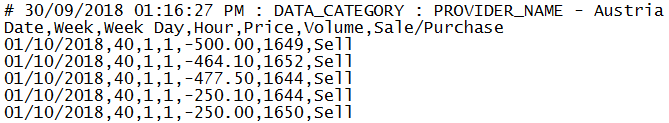
\includegraphics[width=.75\textwidth]{res/etl/epex_ac.PNG}}
        \caption{Metadata in first rows of a \texttt{csv} file.}
        \label{fig:etl:csv:ac}
    \end{figure}
    
    As we can see from Figure \ref{fig:etl:csv:ac}, the first row of the \texttt{csv} file requires special attention.
    
    From it we can extract information about\footnote{
        Some information are under a non-disclosure clause and as such have been anonymized.
    }:
        \begin{itemize}
            \item Creation date \textit{(30/09/2018 01:16:27 PM)}
            \item Category \textit{(DATA\_CATEGORY)}
            \item Provider \textit{(PROVIDER\_NAME)}
            \item Country \textit{(Austria)}
        \end{itemize}
    These information are then appended to each row of the dataset and stored on the Data Warehouse.

\paragraph{Multiple data formats}
    \begin{figure}
        \centering
        \fbox{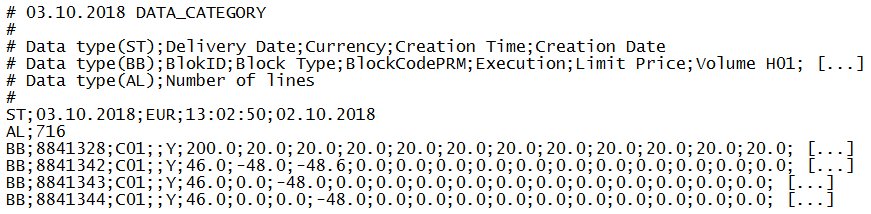
\includegraphics[width=\textwidth]{res/etl/epex_bb.png}}
        \caption{\texttt{Csv} with multiple data formats.}
        \label{fig:etl:csv:bb}
    \end{figure}
    
    For a different data stream, the first 6 rows of the file define some metadata of the dataset, and need to be treated separately.
    Figure \ref{fig:etl:csv:bb} shows the format of the data.
    
    This file contains three different types of data, each with its own format and structure.
    The first rows define the columns available for different types of data.
    The first column of the dataset specifies the data type.
    
    As we can see from Figure \ref{fig:etl:csv:bb}, the first three rows (of type, respectively, \texttt{ST}, \texttt{AL} and \texttt{BB}) have a different number of columns.
    This causes problems when reading the dataset, and requires splitting the file in three datasets, each for a data type.
    
    The first line is, instead, handled similarly to the situation described in the previous example.
    \subsection{Unpredictable File Names} \label{section:etl:terna}
        The website of Terna S.p.A.\footnote{
    Terna S.p.A. is the most important Transmission System Operator in Italy.
    It manages almost all of the Italian energy transmission grid.
} is an example of technical problems which heavily influenced the extraction process.

\paragraph{Premise}
    Terna provides each day an Excel file containing several data.
    An intuitive approach would be to download directly these files.
    
    However, due to the inconsistencies described in the next paragraph, it became necessary to navigate the website with a web scraper, which is far more complex to develop than a simple downloader.
    
\paragraph{Inconsistencies}
    The main problem with the Terna website is that there isn't any naming convention for the Excel files.
    
    As we can see from Table \ref{tab:etl:terna:files}, files related the same data category for consecutive days have both very different names and different extensions.
    Moreover, some files marked as \texttt{.xlsx} are actually just \texttt{.xls} with a wrong file extension.
    
    \begin{table}
        \centering
        \begin{tabular}{|c c c|}
            \toprule
            Date & Filename & Extension \\
            \midrule
            11/04/2019 & 73 & XLS  \\
            10/04/2019 & 52 & XLSX \\
            09/04/2019 & 31 & XLS  \\
            08/04/2019 & 03 & XLS  \\
            \bottomrule
        \end{tabular}
        \caption{
            Filenames and extensions for files downloaded from \texttt{Terna.it}.
            All files are related to the same category.
        }
        \label{tab:etl:terna:files}
    \end{table}
    
  \paragraph{Web scraper}
    Since it is impossible to predict which files to download, the only possible approach is to navigate the website and download the files manually or through a web scraper.
    The downloader uses Selenium to navigate and interact with Terna website, and to retrieves the URLs of several \texttt{.xls} and \texttt{.xlsx} files, which will be downloaded by Databricks.
    
    This process is by far slower than a normal downloader, but allows us to bypass the filename issue.
    \subsection{Website Navigation}
        Damas\footnote{
    Damas is a private web portal managed by Terna S.p.A.
    It provides data related to energy transfers between Italy and bordering countries.
    Information from this website are private, meaning that each company can only see their own energy transfers.
} is an example of a website which requires complex navigation logic.

The website offers a simple interface for selecting a time range and showing the data for that given range.
However, this system presents two limitations.

\paragraph{Limited date range}
    First of all, the maximum date range allowed is 31 days.
    If a user tries to perform a query on a bigger date range, the system shows an error message.
    
    This means that it is necessary to perform 12 queries to download a whole year.

\paragraph{No DST}
    The other problem is that if a date range contains a DST change, the website shows the following error message:

    \begin{center}
        \texttt{
            One of the days in the interval BUSDAY(30.03.2019) and\\ BUSDAYTILL(31.03.2019) contains clock change days.
        }
    \end{center}
    
    As shown by the message, it is impossible to download even a small amount of days, if a DST change occurs between them.

    The solution would be to download these dates individually, while downloading the rest of the data in ranges smaller than 31 days.
    However, since each year has different dates for DST changes, it would be necessary to set up these date manually for each year in the downloader.
    
    In the end, the best solution, even though it's computationally less effective, is to download each day individually.
    In this way there is no need to group dates into ranges and to pay attention to DST changes.
    The download process, on the other hand, is slower than downloading data in a batch.
    
    \chapter{Data Warehouse Structure}
        The data warehouse has been built with a particular structure, suited for both storing and processing the huge amount of data needed, as well as dealing efficiently with its high heterogeneity.

The various schemas created, as well as how they contribute to processing and exposing all the information, will be described in this chapter.
A final section will elaborate on a particular type of tables, which plays a very important role in the Data Warehouse.

\section{Schemas}
    The data warehouse contains several schemas, each one serving a specific purpose.

Two schemas, called \textit{Source} and \textit{Staging}, are used for loading the data, while a different one, called \textit{Data Mart}, contains the final data.

The first two schemas behave differently from the latter, since their purpose is to process the content of each \texttt{csv} file when inserting new data into the Data Warehouse.
These tables are emptied each time a different file is processed.

Several additional schemas, are also present in the data warehouse, but they have a less important role.

\subsection{Source}
    The \textit{Source} schema, named \texttt{src}, is where Databricks directly loads the \texttt{csv} data at the end of the ETL process.
    
    It contains a table for each data stream downloaded by Databricks.
    The structure of these tables is identical to the \texttt{csv} structure.
    All fields are of type \texttt{VARCHAR}, since all values loaded from \texttt{csv} are by default interpreted as strings.
    
    Each table in this schema has associated a view.
    These views are used to cast the data to their correct types as well as rename the fields into a standardized format.
        
\subsection{Staging}
    The \textit{Staging} schema, called \texttt{stg}, loads the data from the \texttt{stg} schema views and performs some more operations on them.
    
    The number of tables in this schema is much lower than the one in the \texttt{src} schema.
    This is because the data in this schema are aggregated together.
    
    \paragraph{Example}
        Let us take for example weather data.
        Information about weather come from several providers.
        Each one has different information: some providers may contain data about temperature and humidity, while others may have information about gas or power demand\footnote{
            These information are correlated.
            For example, on a cold day there is more need for heating and, as a consequence, a higher gas demand.
        }.
        In other cases, for example, a provider may be related to a single zone (e.g., energy consumption in Austria), so multiple providers are needed to get the whole European picture.\\
    
    In all these cases, it is necessary to group together data from different providers, since the information they provide are strictly correlated.
    
    This aggregation is done in this schema by apposite procedures.
    These procedures read data from the views present in the \texttt{src} schema.

\subsection{Data Mart}
    The \textit{Data Mart} schema, called \texttt{dm}, contains the first layer of data to be consulted by users.
    
    Data are loaded into this schema from the \textit{staging} stables.
    
    Tables in this schema are meant to be consulted by end-users for their daily needs.
    Information contained in this schema are both up-to-date and complete (i.e., each table contains data related to several years back and there are no missing values).
    
\subsection{DBO}
    The \texttt{dbo} schema contains remappings, which are used to normalize some data.
    
    Remappings will be described in section \ref{section:dwh:remappings}.

\subsection{Configuration}
    An interesting schema is the one called \texttt{configuration}, which contains some parameters which influence the ETL process executed by Databricks.
    
    Amongst all the parameters, two are of particular interest: the download time range, as well as retry information, in case of download failure.
    Table \ref{tab:dwh:configuration} is an example of configuration parameters stored in this schema.
    
    \begin{table}
        \centering
        \begin{tabular}{|c c|c c|c c|}
            \toprule
             Provider   & Stream      & From       & To   & Retries & Retry Delay \\
             \midrule
             Weather\_A & Temperature & 01/01/2017 & NULL & 3       & 10         \\
             Weather\_A & Humidity    & 01/01/2017 & NULL & 3       & 10         \\
             Weather\_B & Temperature & 01/01/2019 & NULL & 2       & 15         \\
             Weather\_B & Pressure    & 01/01/2018 & NULL & 5       & 5         \\
             \bottomrule
        \end{tabular}
        \caption{Some configuration parameters.}
        \label{tab:dwh:configuration}
    \end{table}
    
    \paragraph{Download time range}
        These information are used to specify when to stop when downloading data from a given provider.
        
        This parameter has two uses: first of all, in case the provider has more historical information than what needed, it limits the amount of data recovered.
        This not only reduces history download time, but also prevents too much unneeded data from being loaded into the data warehouse.
        In the opposite case, this parameter is also needed not to attempt to download historical data from a provider if we know it is not available.
        This prevents the downloader from encountering errors caused by non-existent files.
        
        A \texttt{NULL} value specifies that there is no time range limit.
    
    \paragraph{Retries}
        The downloaders have been programmed to attempt again to download data in case the provider timeouts.
        
        These parameters specify both how many attempts to perform, as well as the required delay between each attempt.
        
        Given the different importance and update frequency of the different providers, these values differ depending on which data is being downloaded.
    
    \paragraph{Remarks}
        It is important to notice that these parameters are not specified for each provider, but for each data stream.
        
        This decision has been made considering two factors.
        
        First of all, sometimes data from a single provider is recovered from multiple sources (e.g. different websites belonging to the same organization).
        Each source can present a different level of availability.
        
        Secondly, some data streams are more important than others.
        It is reasonable to spend more effort downloading this kind of data if they happen to be unavailable, otherwise some critical processes may stop working.

\subsection{Other Schemas}
    The Data Warehouse contains also other schemas, which play, however, a less important role in the data processing procedures.
    
    For example, the schema \texttt{trd} (\textit{Trading}) contains some views explicitly requested by the trading team.
    These views are just a simple manipulation of the data stored in the \textit{Data Mart} schema.
    Their purpose is exposing some data in a particular format, which is required by some tools used by the trading department.
    

    
\section{Remappings} \label{section:dwh:remappings}
    Some information can be expressed in different ways.

For example, the same hour can have different values depending on the timezone used.
Some providers also count hours from 0 to 23, while others use the most common 1-24 notation.

When dealing with this kind of data, it is important to choose a consistent and uniform way of these information.

This action is done through additional tables, used to remap the original data to the uniform notation used.

\subsection{Logic vs Materialized Remappings}
    Remappings can be either logical or materialized.

The former are created by joining any table with a remapping table, producing the results in the query output.
In the latter case, on the other hand, the results are physically stored on the data warehouse and do not require any join operation.

Let's now analyze the advantages and disadvantages of each remapping technique.

\subsubsection{Query performance}
    The type of remapping chosen can directly influence the performance of a query.

    \paragraph{Logical remappings}
        Logical remappings require to join each value of a given table with the remapping.
        This operation is applied to a large amount queries used by Axpo, since they require some information in a specific notation.
        
        The cost of the join is however low, since these remapping tables are usually very small, ranging from tens to a couple hundred rows.
        As such a single join can be computed very quickly, but it can become a problem if these operations need to be applied for almost each query.
        
    \paragraph{Materialized remappings}
        Materialized remappings require no additional overhead, since the remapped information are physically stored along the other data.
        
        This choice is ideal for values which are always used in their remapped notation.
        For example, each provider uses its own hour notation, while all Axpo tools use a standard numeric notation ranging from 1 to 25.
        
        Instead of having to perform a join for \textunderscore{every} query, it is more efficient to memorized this value directly into the table, removing the join overhead.
    
    
\subsubsection{Query complexity}
    Queries become more complex since they require join operations with additional tables.
    This scenario is even more complex when multiple remappings are needed for the same table.
    
    \paragraph{Logical remappings}
        For local remappings, each remapping needed results in a join operation.
        
        Sometimes, multiple columns referring to the same type of information need to be remapped.
        This leads to a more complex query, in which it is necessary to remember the name of each remap in order to avoid confusion.
        
        \begin{figure}
            \centering
            \begin{subfigure}{\textwidth}
                \centering
                \fbox{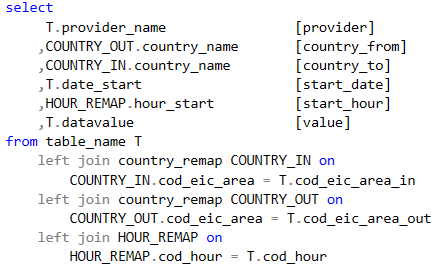
\includegraphics[width=.5\textwidth]{res/dwh/remap_logical.png}}
                \subcaption{Logical}
                \label{fig:dwh:remapping:complexity:logical}
            \end{subfigure}
            
            \begin{subfigure}{\textwidth}
                \centering
                \fbox{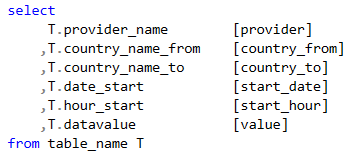
\includegraphics[width=.4\textwidth]{res/dwh/remap_materialized.png}}
                \subcaption{Materialized}
                \label{fig:dwh:remapping:complexity:materialized}
            \end{subfigure}
            
            \caption{Query complexity for different remappings. Both queries produce the same output.}
            \label{fig:dwh:remapping:complexity}
        \end{figure}
        
        As an example, the query shown in Figure \ref{fig:dwh:remapping:complexity:logical} represents a query using logical remappings.
        As we can see, multiple join operations are needed, making the query harder to read.
        
    \paragraph{Materialized remappings}
        Materialized remappings do not need any join operation, since the data is directly present in the table.
        As a consequence, queries are both easier to write and to read.
    
        The query shown in Figure \ref{fig:dwh:remapping:complexity:materialized} represents the same query as above, but uses materialized remappings.
        The query is certainly easier to read and to understand, and the possibility of making errors is minimized.

\subsubsection{Data insertion}
    When a new row is inserted additional operations have to be performed depending on the remapping type.
    
    \paragraph{Logical remappings}
        Logical remappings are more convenient during insertion, since they do not require any additional operation on the values inserted.
        
        The only check needed is that each value to be remapped is present in the remapping table.
        
        Otherwise an alert must be raised and an appropriate remapping has to be created.
    
    \paragraph{Materialized remappings}
        In case of materialized remappings, it is necessary to compute each remapping prior to the insertion operation.
        
        In case of missing values, there are two possibilities: either the row is not inserted or it is inserted with a temporary remapped value of \texttt{NULL}.
        In both cases an alert must be raised.

\subsubsection{Remapping changes}
    Remapping tables can be changed if errors are detected.
    Depending on the remapping type used for a specific values, different scenarios may occur.

    \paragraph{Logical remappings}
        Logical remappings handle changes to remapping tables very efficiently.
        
        Since the remapped value is computed at query time, no additional operation are needed on the table.
        
    \paragraph{Materialized remappings}
        Materialized remappings need to be updated each time the remapping table is modified.
        
        All remapped values are computed again by an apposite procedure (the same used during insertion).
        In case of incomplete remappings (e.g., a value from the remapping table has been removed), an alert must be raised.

\subsection{Examples}
    In this section, I will provide a few examples of the remappings created by Reply, to give a more hands-on idea of the notations used by different providers, as well as how they have been normalized.
    
Since I was constantly analyzing the Data Warehouse, I often noticed several small problems with remappings, such as wrong associations or missing values.
Each time I noticed a problem, I analyzed the cause and told Reply how to fix the issue.

In other cases, I directly asked Reply to remap additional data, which could be used to improve query performance or to simplify existing queries.

\subsubsection{Hours}
    \input{tex/chapters/2_solution/dwh/remappings/types/hour.tex}
    
\subsubsection{Countries}
    \input{tex/chapters/2_solution/dwh/remappings/types/country.tex}
    
\subsubsection{Bidding Operation Types}
    \input{tex/chapters/2_solution/dwh/remappings/types/op_type.tex}

% \subsubsection{Granularity / Estimation Period}
%     \input{tex/chapters/2_solution/dwh/remappings/types/granularity.tex}

